%*****************************************
\chapter{Implementation}\label{ch:implementation}
%*****************************************

Um die Webanwendung platformübergreifend entwickeln und auf beliebigen Systemen einsetzen zu können würde ASP.NET Core MVC als Development Framework gewählt.

\section{ASP.NET Core MVC}

Die General-Purpose-Development-Platform .NET Core wurde unter Koordination von Microsoft zusammen mit der .NET Community entwickelt und als Open Source-Projekt über GitHub \cite{dotnetcore} verfügbar gemacht. Sie bietet eine platformübergreifende Lösung zur Entwicklung und Ausführung von Anwendungsprogrammen und läuft unter Windows, macOS and Linux. ASP.NET steht für Active Server Pages .NET und ist ein Web Application Framework von Microsoft, mit dem sich dynamische Webseiten, Webanwendungen und Webservices entwickeln lassen. ASP.NET Core MVC baut auf .NET Core auf und vereint die Effektivität und Übersichtlichkeit der Model-View-Controller (MVC) Architektur \cite{freeman2016pro}. Als Entwicklungsumgebung wurde Visual Studio Code, ein kostenloser und quelloffener Texteditor, mit C\# Extension genutzt.

\subsection{Model-View-Controller}

Das Model-View-Controller Design Pattern dient der Trennung der Software in die drei Komponenten

\begin{itemize}
	\item Models, die die Daten enthalten mit denen der Nutzer arbeitet
	\item Views, die Teile des Models rendern und so das User Interface darstellen 
	\item Controllers, die eingehende Anfragen annehmen und Operationen auf dem Model durchführen sowie Views die gerendert werden sollen auswählen
\end{itemize}

Allgemein kann man sagen, dass das model die Objekte der realen Welt repräsentiert, zusammen mit den Prozessen und Regeln die das  bestimmte Einsatzgebiet der App definieren. Dies wird auch als Domain der Applikation bezeichnet und analog wird das Model auch Domain Model genannt. Die C\#-Models zusammen mit ihren Methoden bilden die Wirklichkeit auf die Applikation ab. Dabei stellen die Views zusammen mit den Controllern die Domain dem Client dar.



Dabei ist jeder Teil der MVC Architektur eigenständig und wird auch `separation of concerns' genannt. So werden die Daten im Model ausschließlich vom Model verändert, die Daten ausschließlich vom View dargestellt und user requests und input ausschließlich im Controller verarbeitet. Durch diese klare Trennung der Komponenten wird es einfacher die Application zu warten und zu erweitern. Der Zusammenhang zwischen den einzelnen Komponenten ist in Abbildung \ref{fig:mvc} dargestellt.

\begin{figure}
\centering
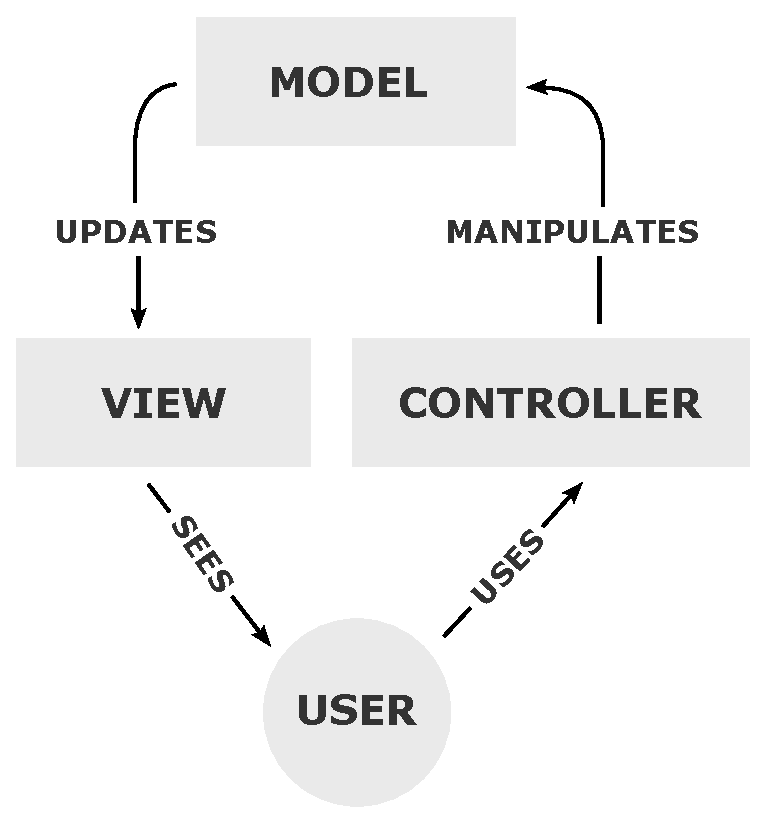
\includegraphics[width=6cm]{Figures/mvc}
\caption{Model-View-Controller}
\label{fig:mvc}
\end{figure}

 Beim MVC-Pattern werden eingehende Anfragen durch Controller behandelt. In ASP.NET Core MVC sind Controller C\#-Klassen die gewöhnlich von der integrierten MVC-Controller Basisklasse \code{Microsoft.AspNetCore.Mvc.Controller} erben. Jede \code{public}-Methode eines Controllers wird auch \emph{action method} genannt. Man kann sie aus dem Web über eine URL aufrufen und so eine Aktion ausführen. In einer Web Application geht es darum dynamischen Output zu konstruieren und darzustellen. In MVC ist der Controller dafür zuständig basierend auf dem Model Daten zu konstruieren und diese an den View weiterzugeben, welcher wiederum das HTML rendert. Wenn also eine Anfrage an die URL die mit der action method verbunden ist gesendet wird, werden die Statements in der action method ausgeführt um Operationen auf domain model anzuwenden und dann ein view auszuwählen der dem Client angezeigt wird. Dies is in Abbildung \ref{fig:mvc_http} dargestellt.
 
 
 \begin{figure}
\centering
\includegraphics[width=\textwidth]{Figures/mvc_http}
\caption{HTTP request mit Model-View-Controller}
\label{fig:mvc_http}
\end{figure}
 
 
\subsection{Routes}

ASP.NET Core MVC Applications nutzen das ASP.NET routing system. Diese entschiedet welche URLs auf welchen Controller und welche Actions abgebildet werden. Eine Route ist eine Regel die darüber entscheidet wie eine Anfrage behandelt wird. Als Standardregeln für ein neues MVC Projekt sind werden beispielsweise die folgenden URLs auf die Index action des code{HomeControllers}s weitergeleitet.

\begin{itemize}

	\item /
	\item /Home
	\item /Home/Index

\end{itemize}

\noindent
Nach Konvention hat die Application einen \code{HomeController} welcher den Einstiegspunkt in die MVC Application bildet.


\subsection{Razor View Engine}

Für eine Webapplikation ist es essentiell dynamischen Inhalt zu generieren und an den Client zu senden. Die Razor View Engine ist eine ASP.NET template markup syntax die zur dynamischen Erstellung von Webseiten in C\# genutzt wird \cite{razorengine}. Dabei sind Razor views HTML templates die C\#-Logik enthalten, welche model data nutzt um dynamisch Content zu generieren. Weil Razor Expressions fast jedes gültige C\#-Statement enthalten können ist es mitunter schwierig zu entscheiden ob Logik in den View oder in den Controller gehört ohne das MVC pattern zu untergraben.

\subsection{Model Binding}

Model Binding ist ein nützliches Feature von MVC. Eingehende Daten eines HTTP-requests werden geparsed und unter Berücksichtigung der Key-Value-Pairs den Properties des jeweiligen domain models types zugewiesen. Dadurch wird das mühevolle Behandeln von HTTP requests vermieden und man kann direkt mit C\# Objekten arbeiten anstatt mit Datenpaketen die vom Browser gesendet werden.

\subsection{Tag Helper}

\section{Entity Framework Core}

Entity Framework (EF) Core is a lightweight, extensible, and cross-platform version of the popular Entity Framework data access technology.
EF Core is an object-relational mapper (O/RM) that enables .NET developers to work with a database using .NET objects. It eliminates the need for most of the data-access code that developers usually need to write. EF Core supports many database engines, see Database Providers for details. 

With EF Core, data access is performed using a model. A model is made up of entity classes and a derived context that represents a session with the database, allowing you to query and save data. See Creating a Model to learn more.
You can generate a model from an existing database, hand code a model to match your database, or use EF Migrations to create a database from your model (and evolve it as your model changes over time).

Instances of your entity classes are retrieved from the database using Language Integrated Query (LINQ). 

Entity Framework Core uses Language Integrate Query (LINQ) to query data from the database. LINQ allows you to use C\# (or your .NET language of choice) to write strongly typed queries based on your derived context and entity classes. A representation of the LINQ query is passed to the database provider, to be translated in database-specific query language (e.g. SQL for a relational database).\cite{msentitiyframework}


Entity Framework Core is able to generate the schema for the database using the model classes through
a feature called migrations. When you prepare a migration, EF Core creates a C\# class that contains the SQL commands required to prepare the database. If you need to modify your model classes, then you can create a new migration that contains the SQL commands required to reflect the changes. In this way, you don’t have to worry about manually writing and testing SQL commands and can just focus on the C\# model classes in the application.\cite{dotnetcore}

\section{CSV-Reader}

The CsvReader library is an extended version of Sébastien Lorion's fast CSV Reader project and provides fast parsing and reading of CSV files \cite{csvreader}.

\section{SQLite}

SQLite is an in-process library that implements a self-contained, serverless, zero-configuration, transactional SQL database engine. The code for SQLite is in the public domain and is thus free for use for any purpose, commercial or private. SQLite is the most widely deployed database in the world with more applications than we can count, including several high-profile projects.

SQLite is an embedded SQL database engine. Unlike most other SQL databases, SQLite does not have a separate server process. SQLite reads and writes directly to ordinary disk files. A complete SQL database with multiple tables, indices, triggers, and views, is contained in a single disk file. The database file format is cross-platform - you can freely copy a database between 32-bit and 64-bit systems or between big-endian and little-endian architectures. These features make SQLite a popular choice as an Application File Format. Think of SQLite not as a replacement for Oracle but as a replacement for fopen() \cite{sqlite}


\section{Bootstrap}

